\documentclass{article}
\usepackage[a4paper, margin=2.5cm]{geometry}
\usepackage{amsmath}
\usepackage{caption}
\usepackage{placeins}
\usepackage{graphicx}
\usepackage{subcaption}
\usepackage{setspace}
\doublespacing
%\usepackage[active,tightpage]{preview}
\usepackage{natbib}
\bibpunct{(}{)}{,}{a}{}{;} 
\usepackage{url}
\usepackage{nth}
\usepackage{authblk}
% for the d in integrals
\newcommand{\dd}{\; \mathrm{d}}
\newcommand{\tc}{\quad\quad\text{,}}
\newcommand{\tp}{\quad\quad\text{.}}
\defcitealias{HMD}{HMD}

\newcommand\ackn[1]{%
  \begingroup
  \renewcommand\thefootnote{}\footnote{#1}%
  \addtocounter{footnote}{-1}%
  \endgroup
}
\begin{document}

\title{Macro patterns in the shape of aging}

\author[1]{Tim Riffe\thanks{riffe@demogr.mpg.de}}
\author[2,3]{Jos\'e Manuel Aburto}
\affil[1]{Department of Demography, University of California, Berkeley}
\affil[2]{University of Southern Denmark}
\affil[3]{Max Planck Odense Center on the Biodemography of Aging}

\maketitle

\begin{abstract}

\end{abstract}

\section*{Extended abstract}

Typically demographers summarize the distribution of remaining
lifetimes by age using the mean, $e(a)$. However, remaining life
expectancy is not an omnibus descriptor of time to death. There are other
useful measures of longevity, such as the modal or median ages at death, and demographers also have a battery of
indicators for lifespan variability or entropy. One aspect in common for many
such indicators is that they refer to the age distribution of mortality in a snapshot of a stationary population or else the age at death distribution of a newborn cohort under constant mortality
conditions. These measures are not typically made conditional on survival to
later ages, i.e., demographers seldom consider the properties of the
age-conditioned distribution of remaining lifetimes. 

Life expectancy at birth, $e(0)$ is one of the most widely used measures to
summarize population health. Its significant and consistent increase witnessed during the last two centuries is one of the most remarkable achievements of modern societies. Most countries have improved in this indicator, and the most long-lived populations have steadily increased their average length of life by 2.5 years every decade. However, life expectancy conceals uncertainty surrounding lifetimes, a dimension of population health that expresses the ultimate difference in survivorship among individuals. Variation in lifespans has recently arisen as an important dimension in aging and health research since it addresses the growing interest in health inequalities, and its linkage with social behavior. It has been found to be negatively associated with life expectancy levels in several countries and over millions of years of primate evolution. Although the degree of the correlation varies between publications, partly because of the data and measures used, the basic finding of a strong association is supported.  For instance, the joint rise of life expectancy and lifespan equality can be described by a straight line from average lifetimes below three years, during mortality crises such as famines and epidemics, to almost 90 years in the most longlived populations, such as contemporary Japanese women.

\subsection*{Definitions}

Remaining life expectancy conditional on survival to age $a$ is defined as
\begin{equation}
e(a) = \frac{1}{l(a)}\int_0^\infty l(a+y) \dd y \tc
\end{equation}
where $l(a)$ is lifetable survivorship to age $a$.
%Let lifespans for a given birth cohort be measured with the random variable,
%$X$, with distribution $d(X)$, identical to the $d_x$
%column of the lifetable if a radix of 1 is used. We are interested in the
%conditional density function, $f(X-a ~|~ X \ge a)$, which we denote $f(y|a)$,
% where $a$ is age attained and $y$ is remaining years of life, and which is defined as:
Define the
conditional deaths distribution
\begin{equation}
\label{eq:fya}
f(y|a) = \frac{1}{l(a)} \mu(a+y) l(a+y) \tc
\end{equation}
where $\mu(a)$ is the force of mortality at age $a$. $f(y|a)$ is interpreted as
the probability of surviving to and dying at exact age $a+y$ given survival to
age $a$.

The conditional deaths distribution can be described empirically using
quantiles, or other central measures such as the median or the mode, or perhaps more parsimoniously using its moments.
The $n^{th}$ central moment about the conditional mean of $f(y|a)$,
$\eta_n(y|a)$ is defined as:
\begin{equation}
\eta _n(y|a) =  \int_{y=0}^\infty (y-e(a))^n f(y|a) \dd y \tc
\end{equation}
where $\eta_2(y|a)$ gives the variance of remaining lifespan about $e(a)$,
$\sigma^2(y|a)$.\footnote{Compare with \citet{chiang1984life}, Chapter 10,
Equation 6.10, where the author denotes $f(y|a)$ with $Y_\alpha$.}
Survival-conditioned variance is useful information, but it can be deceptive
because lifespan variation is not symmetric around $e(a)$. The
conditional skewness function, $Skew(y|a)$ captures most such variation and can be roughly interpreted in this way. It is defined as
\begin{equation}
\label{eq:skew}
Skew(y|a) = \frac{\eta _3(y|a)}{\sigma(y|a)^3} \tc
\end{equation}
the third standardized moment. The conditional excess
kurtosis of $f(y|a)$, $Kurt(y|a)$, can be defined as
\begin{equation}
\label{eq:kurt}
Kurt(y|a) = \frac{\eta_4(y|a)}{\sigma(y|a)^4}-3 \tp
\end{equation}
The age pattern of kurtosis describes how the peakedness, or the fatness of the
tails of the remaining distribution change over age. %The coefficient of
%variation of remaining lifespan, $CV(y|a)$ is then simply
%\begin{equation}
%CV(y|a) = \frac{\sigma(y|a)}{e(a)} \tp
%\end{equation}
%$CV(y|a)$ is dimensionless and comparable over age, and its reciprocal
%can be thought of as a signal to noise ratio of one's likely remaining
% lifespan, assuming a constant mortality pattern in ages higher than $a$. Other conditional
%measures may also be devised in similar fashion, the most obvious and useful of
%which are quantiles, which we also calculate in the following empirical
% section.

\section*{Data and Methods}
All formulas are discretized to single ages
using standard demographic approximations, and these are implemented in the
\texttt{R} programming language \citep{R}. We then calculate the above measures
for each year, population, and sex in the Human Mortality Database
\citepalias{HMD}. To examine macro patterns in the central and shape measures,
we show a series of bivariate relationships.

\FloatBarrier
\section*{Preliminary Results}
Note: need to arrange these to economize space
\begin{figure}
\caption{Log Keyfitz entropy by average length of life}
\centering
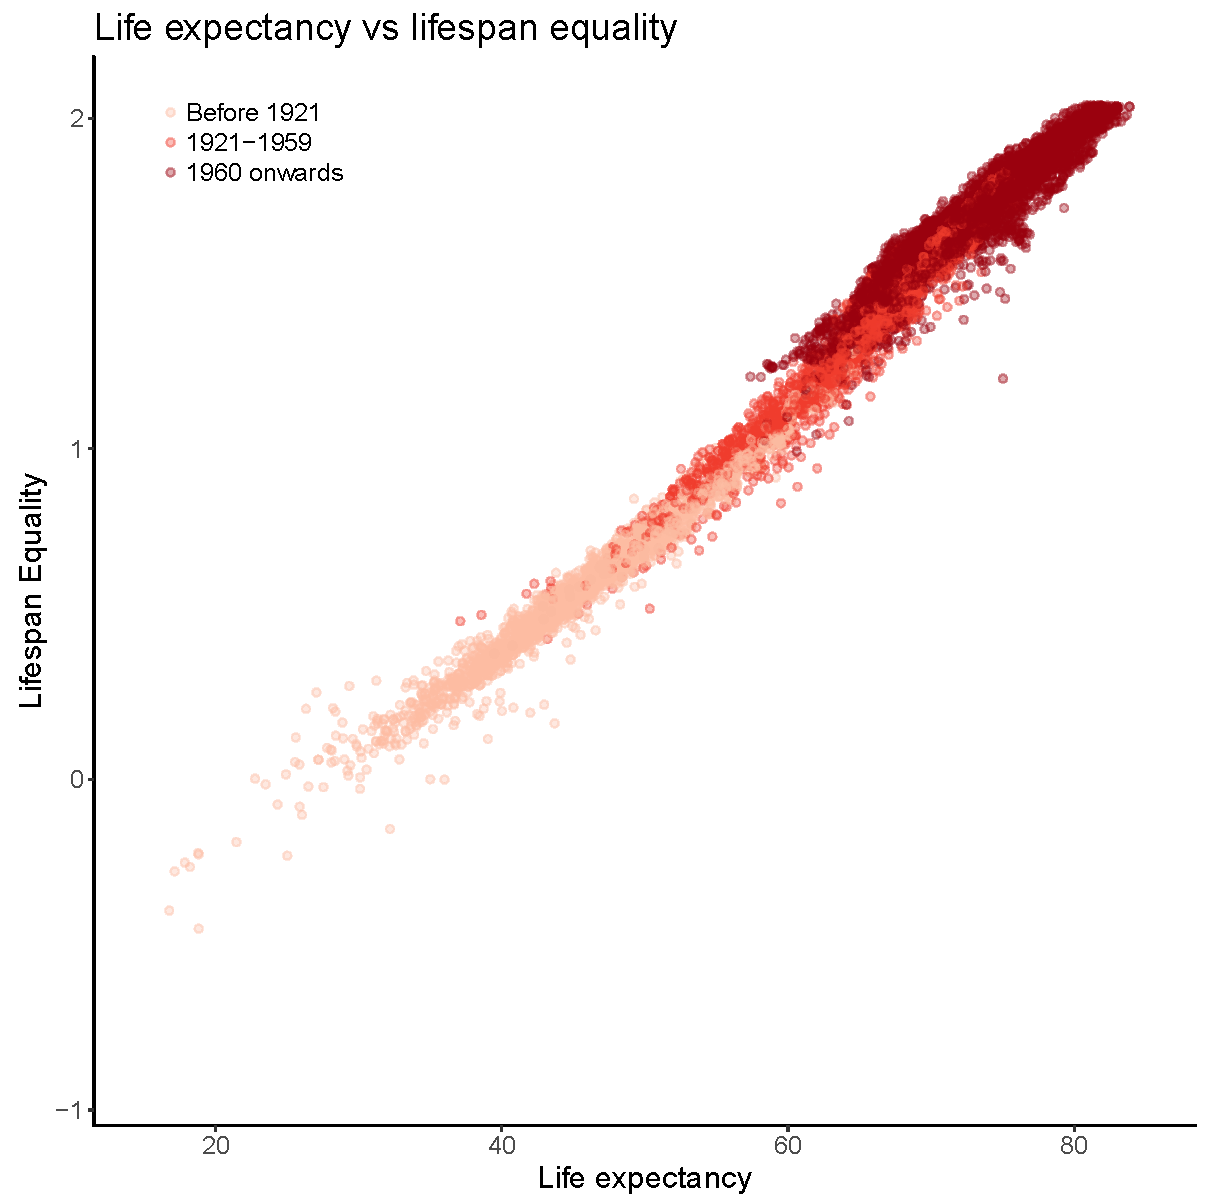
\includegraphics[scale=.5]{Figures/F3_Lifespan_equality}
\end{figure}

\begin{figure}
\caption{Skewness at birth by average length of life}
\centering
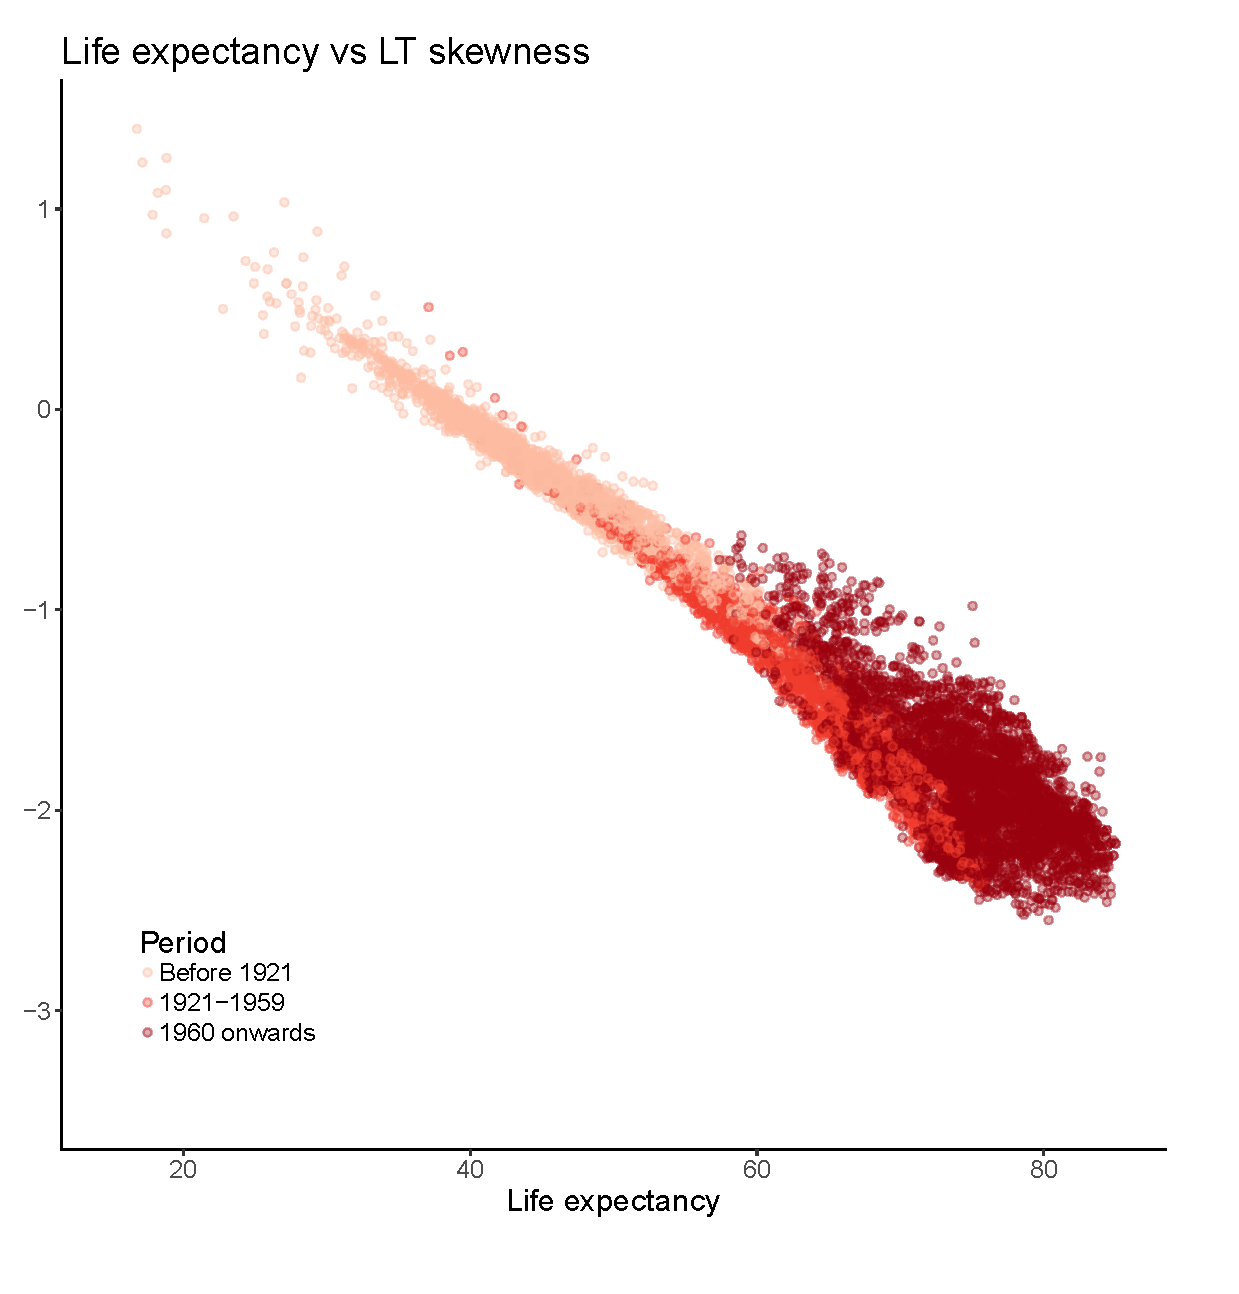
\includegraphics[scale=.5]{Figures/F2_Skew}
\end{figure}

\begin{figure}
\caption{Kurtosis at birth by average length of life}
\centering
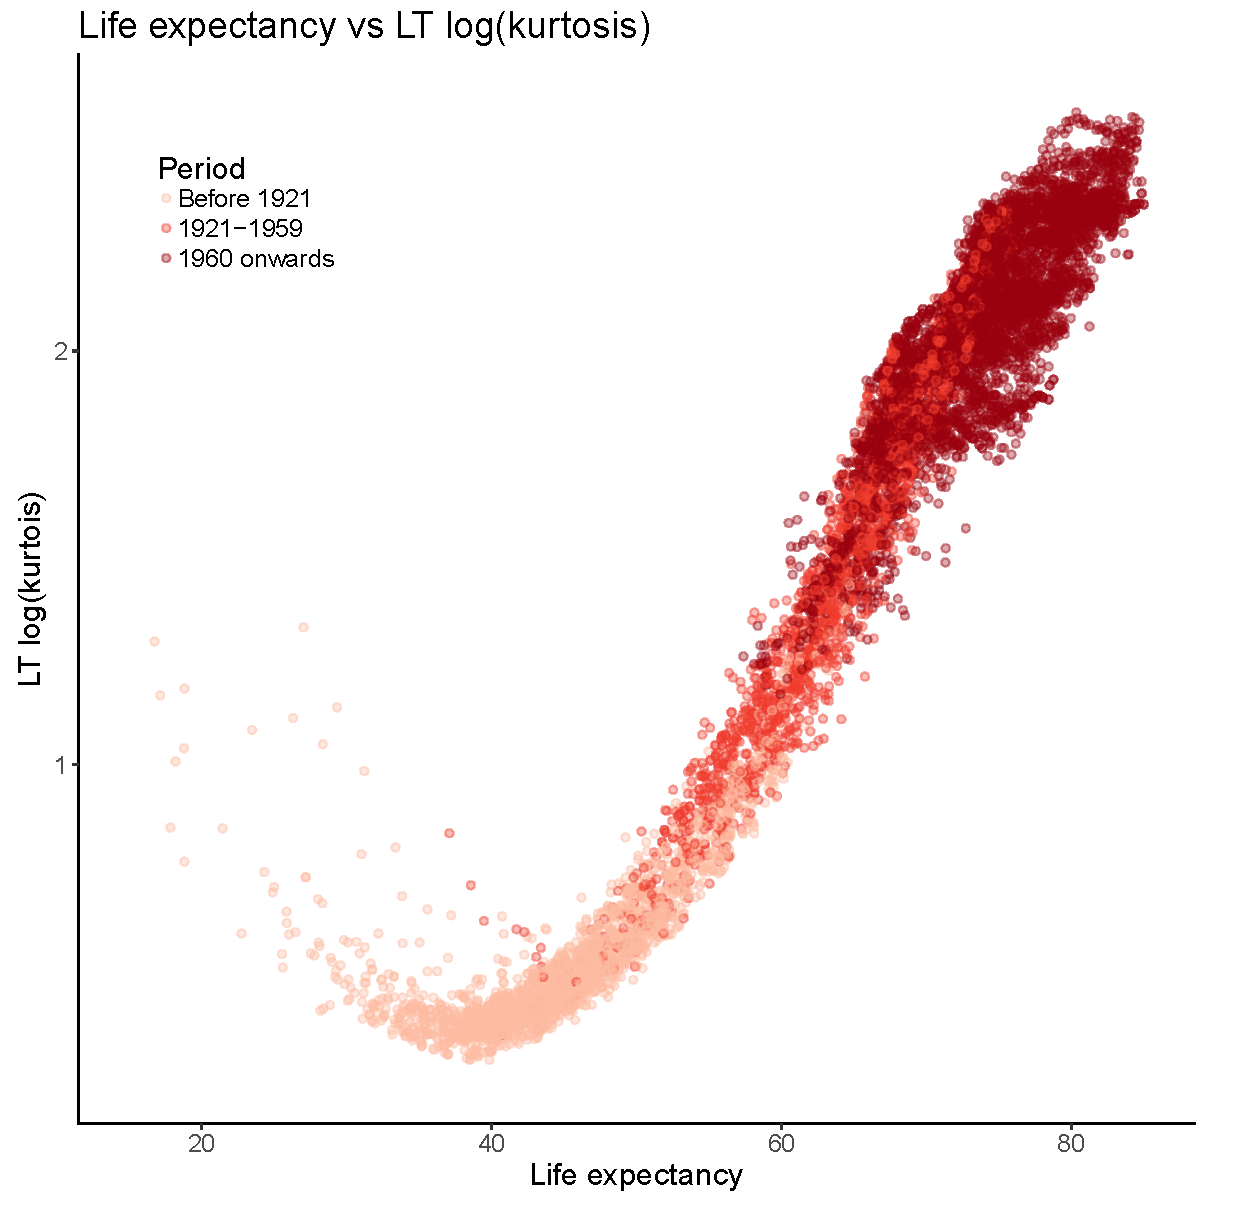
\includegraphics[scale=.5]{Figures/F1_Kurtosis}
\end{figure}

\FloatBarrier
\section*{Discussion}

\bibliographystyle{plainnat}
  \bibliography{references} 

\end{document}
